\documentclass[letterpaper]{article}%
\usepackage{fullpage}[10pt,onesided]%
\usepackage{titlesec}%
\usepackage{amsmath}%
\usepackage{amsfonts}%
\usepackage{enumerate}%
\usepackage{graphicx}%
\usepackage{xspace}%
\usepackage{hyperref}%
\input{tex-util/misc.tex}
\input{tex-util/figures.tex}
\input{tex-util/listings.tex}
\input{tex-util/math.tex}

\date{Friday, May 9th, 2012}
\title{Noweats \\
  {\small \sl A Twitter NLP scraper that answers ``What are New Yorkers eating
  over the past hour?''} \\
  \vspace{2em}
  {\small Prof. Ralph Grishman \\ CSCI-GA.2590-001 - Natural Langauge
  Processing}
}
\author{Brandon Reiss}

\begin{document}
\maketitle

\providecommand{\noweats}{\texttt{noweats}\xspace}
\providecommand{\Noweats}{\texttt{Noweats}\xspace}
\providecommand{\nltk}{\texttt{nltk}\xspace}

\section{Overview}%

\begin{figure}[th!]
  \centering
  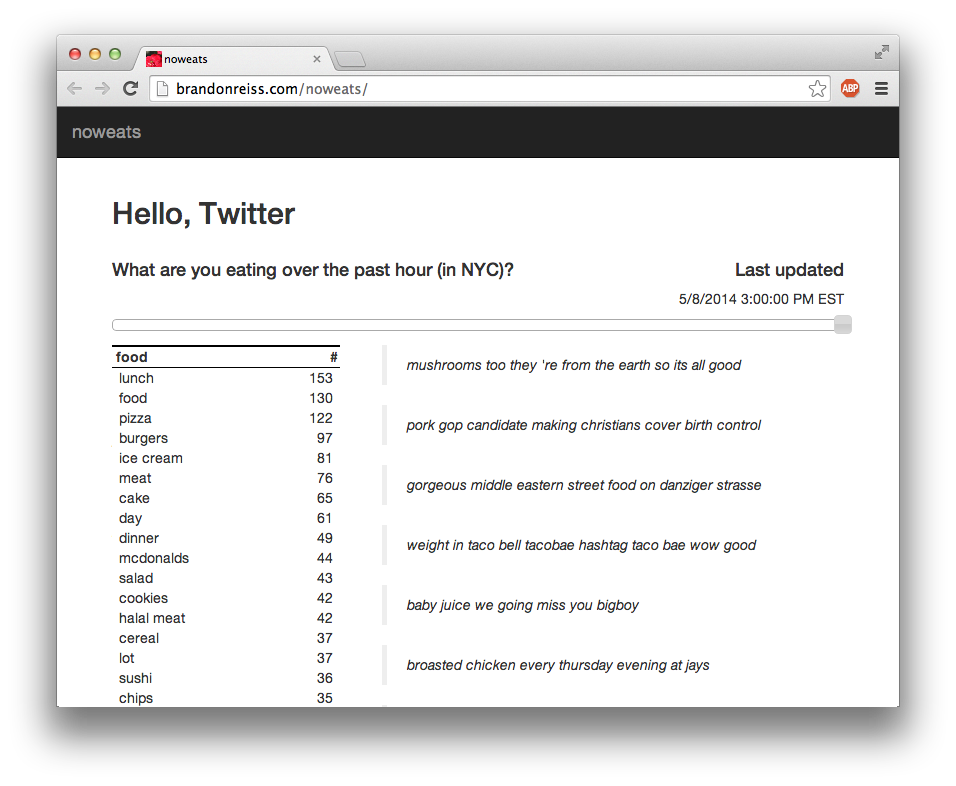
\includegraphics[width=0.8\textwidth]{noweats}
  \caption{Example screenshot of the \noweats page with histogram of top foods
  on the left and listing of top ``interesting'' tweets on the right.}
  \label{fig:noweatsScreenshot}
\end{figure}

\Noweats is an Information Extraction system that cleans, parses, and
aggregates Twitter stream data from New York City to identify foods that people
are eating. It receives apprimately 30,000 tweets per hour using the
\texttt{filter} API tracks [\texttt{ate}, \texttt{eating}, \texttt{eat}] and
the geographical bounding box for NYC. From those tweets, about 20,000 are
eligible for further processing after filtering retweets, user mentions, and
other noise. Of those that are POS tagged, chunked, and scanned, about 6,000
become extracted food items. The final output is merged using an edit distance
heuristic to display the top 200 foods for the hour and a tf/idf score metric
ranks the top 50 ``interesting'' tweets for display next to the food histogram.
See \autoref{fig:noweatsScreenshot} for an example of the \noweats homepage.

All code for \noweats is located at \url{https://github.com/blr246/noweats} and
the front end application is live at \url{http://brandonreiss.com/noweats/}.

\section{Background}%
The NLP task of Information Extraction involves extracting specific data from
an unstructured natural language document. Twitter is a massive source of such
unstructured data and it includes up-to-the-minute accounts of people's
thoughts, desires, actions, and behaviors aggregated by language, locality, and
other discriminating features.

Due to the short format of tweets and the unique linguistic trends adopted by
Twitter users, a stream of tweets is a particularly noisy data source that
includes special slang, abbreviations, unusual Unicode characters, and other
anomalies. A great deal of the \noweats system is devoted to cleaning and
preprocessing tweets so that they may be analyzed by \nltk's POS tagger.

\section{Design}%

\begin{figure}[h]
  \centering
  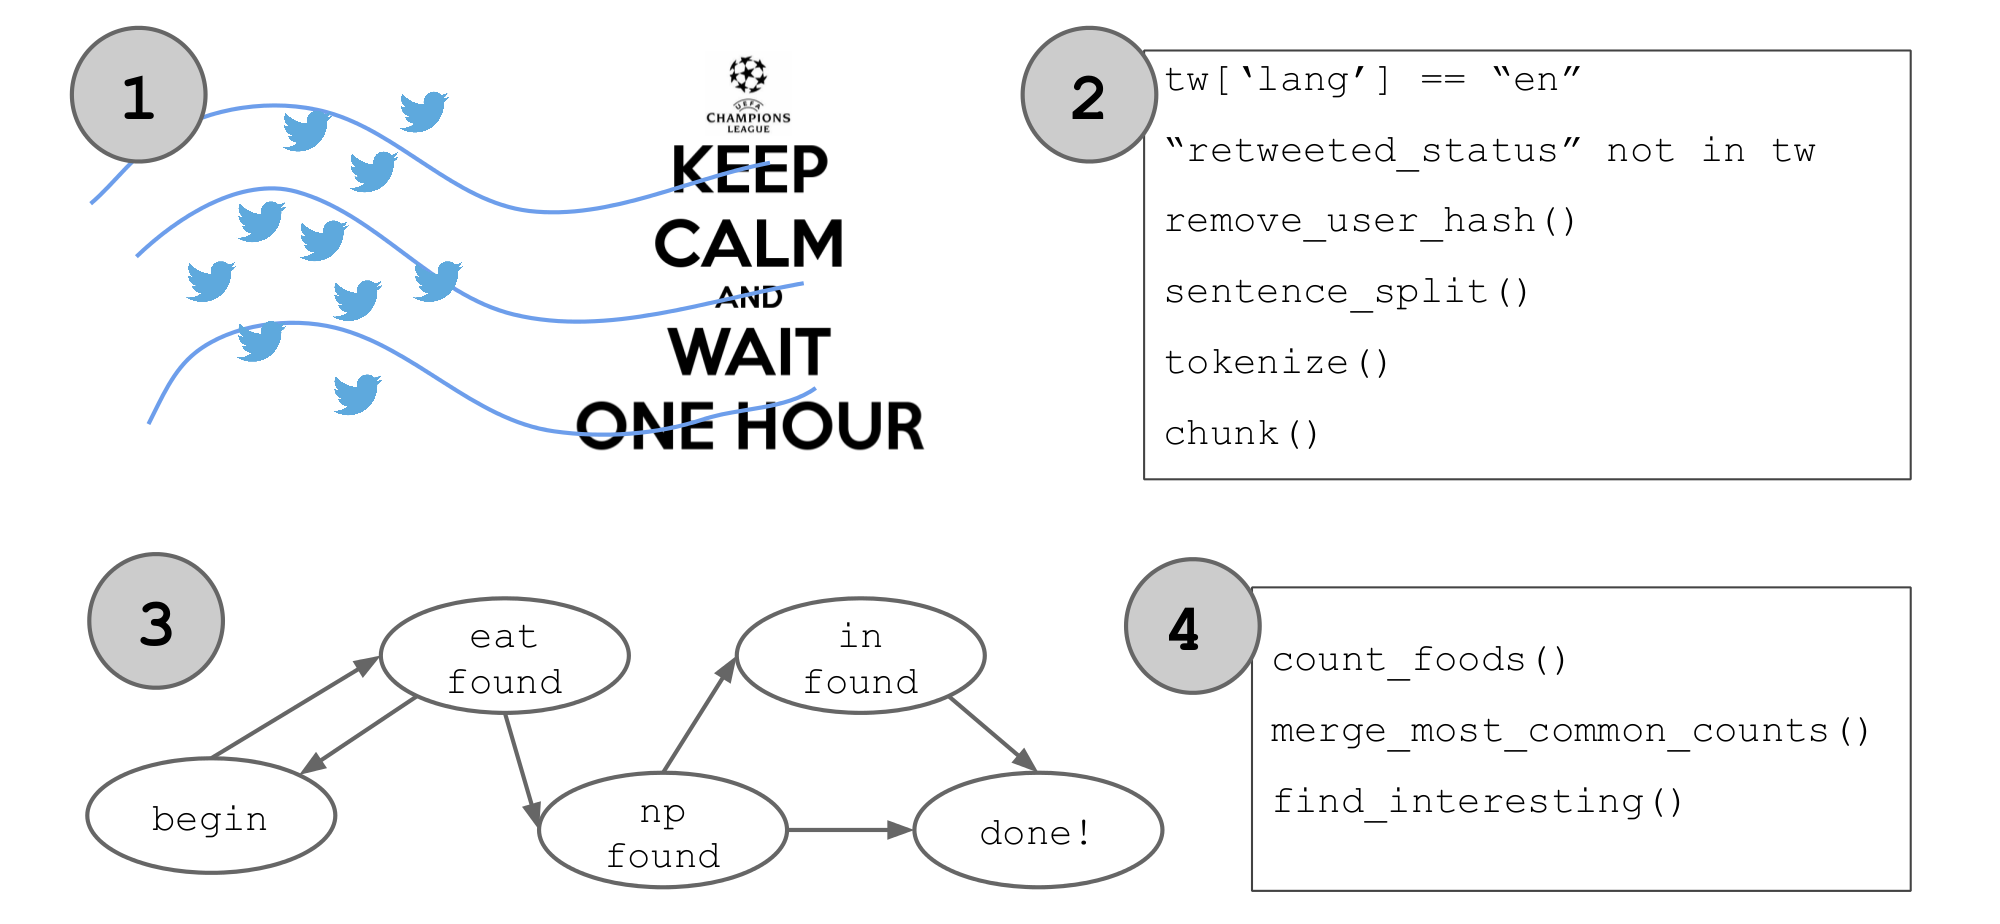
\includegraphics[width=0.8\textwidth]{design}
  \caption{Illustration of the \noweats data pipeline.}
  \label{fig:design}
\end{figure}

The illustration in \autoref{fig:design} describes how data flow from the
Twitter stream to the \noweats front end located at
\url{http://brandonreiss.com/noweats/}. The following is a breakdown of each
step.

\begin{enumerate}[(1)]
  \item \textbf{Collect}: A Python process called \texttt{collect\_nyc}
    streams data from the Twitter API and saves it into log files that roll
    over once per hour. The log files use \texttt{bzip2} compression and
    contain the entire JSON object provided by the Twitter API.

  \item \textbf{Preprocess}: Library functions in the
    \texttt{noweats.extraction} module remove retweets, clean user mentions,
    strip \texttt{\#} characters from hashtags, split sentences, tokenize, POS
    tag, and chunk the data. The chunk grammar is a simple noun phrase
    extractor consisting of sequences of determiners, possessives, adjectives,
    ordinals, and nouns.

  \item \textbf{Scan}: Cleaned, parsed, and chunked tweets are sent through a
    state machine designed to find noun phrases following instances of eat
    verbs. An additional set of states also allows the extraction of
    prepositional phrases or conjunctions immediately following an eat verb
    since these are often useful in specifying the food type. For instance, the
    phrases ``bagel with cream cheese'' and ``peanut butter and jelly'' are
    more illustrative than ``bagel'' and ``peanut butter'' alone.

  \item \textbf{Analyze}: The raw food phrases are sent to library functions in
    the \texttt{noweats.analysis} module. These functions count foods and
    produce a histogram that may be queried for the top $N$ foods using the
    \texttt{most\_common()} method. Another function merges food phrases with a
    very high degree of similarity as determined by an edit-distance based
    score metric. Lastly, a function collects from the raw food list the most
    ``interesting'' food phrases based on a tf/idf-inspired score metric
    computed against the current hour's dataset. The scoring function prefers
    longer food phrases and any word that has a low occurrence in the dataset.
\end{enumerate}

\autoref{tab:codeArtifacts} gives more detail about the purpose of each library
module and script. Note that the entire system is configurable by thresholds,
filters, the eat lexicon, and the location.

\begin{table}[h]
  \centering
  \begin{tabular}{llp{8cm}}
    \toprule
    path & type & description \\
    \midrule
    README.md & text & Basic overview of \noweats including installation and
    usage. \\
    setup.py & script & Used to install \noweats. See \texttt{README.md}. \\
    \\
    bin/collect\_nyc & script & Data collection job configured for NYC. \\
    bin/process\_file & script & Process a single input log file to extract
    \texttt{counts} and \texttt{interesting} output files. \\
    bin/process\_new & script & Scan the data collection directory for any
    files not yet processed by \texttt{process\_file} and process them. \\
    bin/recompress\_data & script & Overcome a bug in the Python \texttt{bz2}
    library by using the \texttt{bzip2} command-line tool to re-compress rolled
    over data files. \\
    \\
    conf/filters.conf & conf & Exclusions for vulgar or mundane phrases.. \\
    \\
    noweats/analysis.py & module & Functions for analyzing extracted food
    phrases. \\
    noweats/collection.py & module & Functions for data collection. \\
    noweats/extraction.py & module & Functions for cleaning, parsing,
    and extracting food phrases from raw tweet data. \\
    \\
    upstart/noweats.conf & conf & Used with \texttt{upstart} to create a system
    service for \noweats. \\
    upstart/noweats.sh & scripe & Script run from \texttt{upstart} that
    controls both the data collection process and the \texttt{process\_new}
    polling process. \\
    \bottomrule
  \end{tabular}
  \caption{Overview of \noweats codebase artifacts.}
  \label{tab:codeArtifacts}
\end{table}

\section{Results}%
Due to the volume of data processed by \noweats and its online nature, a
tradition F1-score analysis is not applicable. The system receives too much
novel data and in too great a quantity to have many supervised labels. During
development, the system was tweaked by reading the output in the browser client
and then tweaking the various processing steps to improve the sense of
``relevance'' conveyed by the results.

For the purpose of this document, we report precision scores in the food counts
that are the quotient of the number of true food items counted versus the
number of food items counted.  For the ``interesting'' display, we will report
precision on relevance, which is subjective but defined as phrases that are
nominally about food or food items. An example relevant phrase is \textsl{bbq
buffet with unlimited beer big time skygarden} and an irrelevant phrase is
\textsl{anybody wan na play gta5 black ops}.

\autoref{tab:countPrecision} gives results for count precision and table
\autoref{tab:interestingPrecision} gives results for ``interesting'' tweet
precision.

\begin{table}[h]
  \centering
  \begin{tabular}{lrrrp{4cm}}
    \toprule
    date & \# false positive & \# foods & precision & excluded \\
    \midrule
    2014-05-08\_15 & 669 & 3236 & 79.33\% &
    {\tiny \texttt{'alone', 'baby', 'bit', 'bitch', 'book', 'booty', 'box',
      'cars', 'children', 'clay', 'contest', 'cum', 'day', 'dirt', 'disorders',
      'doe', 'dog', 'drank', 'face', 'feelings', 'free', 'girl', 'habits', 'hair',
      'half', 'hand', 'hat', 'heart', 'homework', 'hour', 'last night', 'loads',
      'lot', 'makes', 'makeup', 'man', 'money', 'pain', 'people', 'piece', 'pieces
      of', 'right', 'stuff', 'things', 'tho', 'till', 'time', 'wats', 'way', 'week',
      'whatever', 'whole bag', 'whole thing', 'wit', 'words', 'yours'}
    } \\
    \\
    2014-05-08\_07 & 522 & 2057 & 74.62\% &
    {\tiny \texttt{'alone', 'atm', 'beauty', 'bit', 'booty', 'box', 'brother',
      'cardboard', 'cat', 'clay', ``cute 'raina'', 'day', 'dis', 'disorders',
      'dog', 'feelings', 'flowers', 'guy', 'half', 'hat', 'heart', 'im home',
      'insides', 'kaledress', 'last night', 'left', 'life', 'listen now',
      'lot', 'makes', 'makeup', 'man', 'panadol', 'people', 'phone', 'plan',
      'readybrek', 'skills', 'sleep', 'sleep rave repeat', 'someone', 'souls',
      'stuff', 'teaspoon of clay', 'things', 'tho', 'til', 'times', 'tweet',
      'way', 'whatever', 'words', 'wtf'}
    } \\
    \bottomrule
  \end{tabular}
  \caption{Precision results for some selected \texttt{counts} files.}
  \label{tab:countPrecision}
\end{table}

\begin{table}[h]
  \centering
  \begin{tabular}{lrrr}
    \toprule
    date & \# irrelevant & total & precision \\
    \midrule
    2014-05-08\_15 & 17 & 50 & 66\% \\
    2014-05-08\_07 & 13 & 50 & 74\% \\
    \bottomrule
  \end{tabular}
  \caption{Precision results for some selected \texttt{interesting} files.}
  \label{tab:interestingPrecision}
\end{table}

The precision results are in the seventy percent range for both tasks. This
makes the page both useful and entertaining as-is. There are several issues
that affect the results:

\begin{enumerate}[i]
  \item Tweets tend to be trendy so the same joke, meme, or spam will tend to
    accumualte in the results.
  \item The extraction phases are kept simple on purpose in order to allow
    novelty to enter the system. This makes it very difficult to discern the
    phrase ``all day'' from a useful one like ``three pizzas''. This is how
    items like ``all'' enter the final counts.
  \item There are some non-eating uses of the food verbs such as general
    statements about ``eating disorders'' that are also difficult to filter
    apart from useful nouns.
  \item Vulgar language is varied and very common in the dataset. Simple
    filters remove a majority of it, but we don't want to eliminate any tweet
    with a flagged term since there may also be useful food phrases there.
    Sometimes a skeleton of a very vulgar tweet will remain and get presented
    in the results.
\end{enumerate}

Future directions may build up filters over sliding windows in order to find
memes or spam. In addition, a classifier such as a Naive Bayes model could
assist with detecting vulgar content in the interesting list. Wordnet and other
sources could provide a food lexicon to filter some of the results such as
``day''.  With any filtration feature, it would be necessary to tweak
thresholds to avoid a system that is too strict and therefore misses novel
content. Instead, such filters could downweight the count of uncertain content
so that it will be less likely to make the top 200 unless it becomes a stronger
signal.

\end{document}
